% ### Uses XeLaTeX ### %
% ### Needs beamer-master ### %
\documentclass[aspectratio=169]{beamer} %. Aspect Ratio 16:9
\usetheme{AI2} % beamerthemeSprace.sty
% DATA FOR FOOTER
\date{2019}
\title{}
\author{}
\institute{Advanced Institute for Artificial Intelligence (AI2)}
\begin{document}    
% ####################################
% FIRST SLIDE 						:: \SliTit{<Title of the Talk>}{<Author Name>}{<Intitution>}
% SLIDE SUB-TITLE					:: \SliSubTit{<Title of the Chapter>}{<Title of the Section>}
% SLIDE WITH TITLE 					:: \SliT{<Title>}{Content}
% SLIDE NO TITLE 						:: \Sli{<Content>} 
% SLIDE DOUBLE COLUMN WITH TITLE 	:: \SliDT{<Title>}{<First Column>}{<Second Column>}
% SLIDE DOUBLE COLUMN NO TITLE 		:: \SliD{<First Column>}{<Second Column>}
% SLIDE ADVANCED WITH TITLE 			:: \SliAdvT{<Title>}{<Content>}
% SLIDE ADVANCED  NO TITLE 			:: \SliAdv{<Content>}
% SLIDE ADVANCED DOUBLE TITLE 		:: SliAdvDT{<Title>}{<First Column>}{<Second Column>}
% SLIDE ADVANCED DOUBLE NO TITLE 	:: SliAdvD{<First Column>}{<Second Column>}
% ITEMIZE 							:: \begin{itemize}  \IteOne{1st Level} \IteTwo {2nd Level} \IteThr{3rd Level} \end{itemize}
% SECTION 							:: \secx{Section} | \secxx{Sub-Section}
% COLOR BOX 						:: \blu{blue} + \red{red} + \yel{yellow} + \gre{green}
% FRAME 							:: \fra{sprace} \frab{blue} \frar{red} + \fray{yellow} + \frag{green}	
% REFERENCE						:: \refer{<doi number>}
% FIGURE 							::  \img{X}{Y}{<scale>}{Figures/.png} 
% FIGURE							:: \begin{center}\includegraphics[scale=<#>]{Figures/.png}\end{center}
% PROJECT STATUS					:: \planned\~    \started\~   \underway\~   \done\~   
% EXERCICIO							:: \Exe{<#>}{<text>}
% STACKREL							:: \underset{<down>}{<up>}
% FLUSH LEFT						:: \begin{flalign*}  & <1st equation> & \\  & <12nd equation>  & \\ \end{flalign*}
% REAL / IMAGINAY					:: \Re / \Im
% SLASH								:: \sl{} or \sl
% BOLD MATH							:: \pmb{<>}
% ####################################
%
% FIRST SLIDE :: DO NOT BREAK LINE !!!
\SliTit{Git}{Advanced Institute for Artificial Intelligence}{https://advancedinstitute.ai}

% SLIDE WITH TITLE
\SliT{Sumário}{

\begin{itemize}
      \IteOne{Git}
 \end{itemize}

}

\SliT{Git}{

\begin{itemize}
    \IteOne{Projetado para fazer o controle de versão no kernel do Linux}
    \IteOne{Objetivos do Git:}
    \IteOne{Rapidez}
    \IteOne{Suporte para desenvolvimento não linear (milhares de ramos paralelos)}
    \IteOne{Totalmente distribuído}
    \IteOne{Capaz de lidar com grandes projetos com eficiência}
\end{itemize}
}

\SliT{Git}{

\begin{itemize}
    \IteOne{Git website: http://git-scm.com/}
    \IteOne{Livro online: http://git-scm.com/book}
    \IteOne{Página de Referência: http://gitref.org/index.html}
    \IteOne{Tutorial: http://schacon.github.com/git/gittutorial.html}
    \IteOne{At command line: (where verb = config, add, commit, etc.)}
 \end{itemize}
}

\SliT{Git}{

\begin{itemize}
      \IteOne{Repositórios}
      \IteOne{Atualizar arquivos}
      \IteOne{Criando Branches}
 \end{itemize}

}

\SliT{Git}{

Comandos Git:
\begin{itemize}
      \IteOne{git add}
      \IteOne{git commit}
      \IteOne{git push}
 \end{itemize}

}

\SliT{Git}{

\begin{center}
    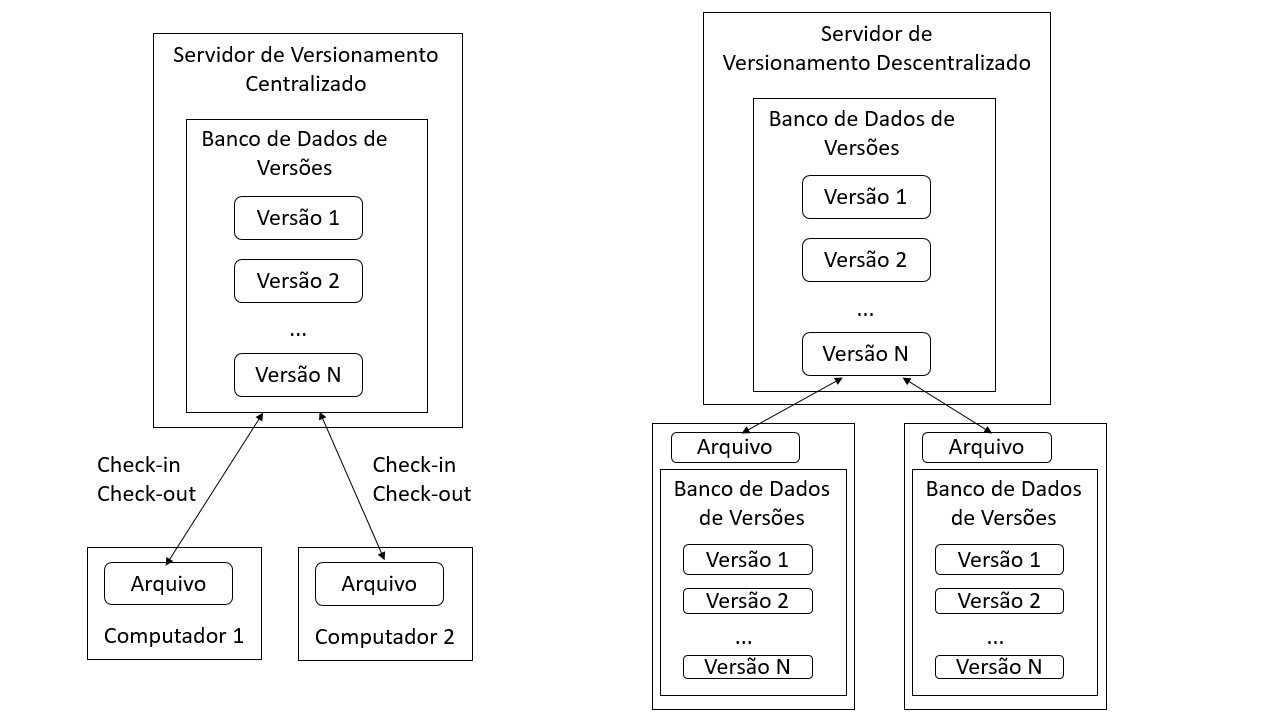
\includegraphics[scale=0.35]{Slide3.jpg}     
    \end{center}
}

% SLIDE NO TITLE
\Sli{
\secx{Dúvidas}

}

\end{document}
